\let\negmedspace\undefined
\let\negthickspace\undefined
\documentclass[journal,12pt,twocolumn]{IEEEtran}
\usepackage{cite}
\usepackage{amsmath,amssymb,amsfonts,amsthm}
\usepackage{algorithmic}
\usepackage{graphicx}
\usepackage{textcomp}
\usepackage{xcolor}
\usepackage{txfonts}
\usepackage{listings}
\usepackage{enumitem}
\usepackage{mathtools}
\usepackage{gensymb}
\usepackage[breaklinks=true]{hyperref}
\usepackage{tkz-euclide} % loads  TikZ and tkz-base
\usepackage{listings}
\usepackage{float}
\newtheorem{theorem}{Theorem}[section]
\newtheorem{problem}{Problem}
\newtheorem{proposition}{Proposition}[section]
\newtheorem{lemma}{Lemma}[section]
\newtheorem{corollary}[theorem]{Corollary}
\newtheorem{example}{Example}[section]
\newtheorem{definition}[problem]{Definition}
\newcommand{\BEQA}{\begin{eqnarray}}
\newcommand{\EEQA}{\end{eqnarray}}
\newcommand{\define}{\stackrel{\triangle}{=}}
\theoremstyle{remark}
\newtheorem{rem}{Remark}
\parindent 0px

\begin{document}
%
\providecommand{\pr}[1]{\ensuremath{\Pr\left(#1\right)}}
\providecommand{\prt}[2]{\ensuremath{p_{#1}^{\left(#2\right)} }}        % own macro for this question
\providecommand{\qfunc}[1]{\ensuremath{Q\left(#1\right)}}
\providecommand{\sbrak}[1]{\ensuremath{{}\left[#1\right]}}
\providecommand{\lsbrak}[1]{\ensuremath{{}\left[#1\right.}}
\providecommand{\rsbrak}[1]{\ensuremath{{}\left.#1\right]}}
\providecommand{\brak}[1]{\ensuremath{\left(#1\right)}}
\providecommand{\lbrak}[1]{\ensuremath{\left(#1\right.}}
\providecommand{\rbrak}[1]{\ensuremath{\left.#1\right)}}
\providecommand{\cbrak}[1]{\ensuremath{\left\{#1\right\}}}
\providecommand{\lcbrak}[1]{\ensuremath{\left\{#1\right.}}
\providecommand{\rcbrak}[1]{\ensuremath{\left.#1\right\}}}
\newcommand{\sgn}{\mathop{\mathrm{sgn}}}
\providecommand{\abs}[1]{\left\vert#1\right\vert}
\providecommand{\res}[1]{\Res\displaylimits_{#1}} 
\providecommand{\norm}[1]{\left\lVert#1\right\rVert}
%\providecommand{\norm}[1]{\lVert#1\rVert}
\providecommand{\mtx}[1]{\mathbf{#1}}
\providecommand{\mean}[1]{E\left[ #1 \right]}
\providecommand{\cond}[2]{#1\middle|#2}
\providecommand{\fourier}{\overset{\mathcal{F}}{ \rightleftharpoons}}
\newenvironment{amatrix}[1]{%
  \left(\begin{array}{@{}*{#1}{c}|c@{}}
}{%
  \end{array}\right)
}
\newcommand{\solution}{\noindent \textbf{Solution: }}
\newcommand{\cosec}{\,\text{cosec}\,}
\providecommand{\dec}[2]{\ensuremath{\overset{#1}{\underset{#2}{\gtrless}}}}
\newcommand{\myvec}[1]{\ensuremath{\begin{pmatrix}#1\end{pmatrix}}}
\newcommand{\mydet}[1]{\ensuremath{\begin{vmatrix}#1\end{vmatrix}}}
\newcommand{\myaugvec}[2]{\ensuremath{\begin{amatrix}{#1}#2\end{amatrix}}}
\providecommand{\rank}{\text{rank}}
\providecommand{\pr}[1]{\ensuremath{\Pr\left(#1\right)}}
\providecommand{\qfunc}[1]{\ensuremath{Q\left(#1\right)}}
	\newcommand*{\permcomb}[4][0mu]{{{}^{#3}\mkern#1#2_{#4}}}
\newcommand*{\perm}[1][-3mu]{\permcomb[#1]{P}}
\newcommand*{\comb}[1][-1mu]{\permcomb[#1]{C}}
\providecommand{\qfunc}[1]{\ensuremath{Q\left(#1\right)}}

\providecommand{\gauss}[2]{\mathcal{N}\ensuremath{\left(#1,#2\right)}}
\providecommand{\diff}[2]{\ensuremath{\frac{d{#1}}{d{#2}}}}
\providecommand{\myceil}[1]{\left \lceil #1 \right \rceil }
\newcommand\figref{Fig.~\ref}
\newcommand\tabref{Table~\ref}
\newcommand{\sinc}{\,\text{sinc}\,}
\newcommand{\rect}{\,\text{rect}\,}
\let\StandardTheFigure\thefigure
\let\vec\mathbf


\bibliographystyle{IEEEtran}


\vspace{3cm}

\title{
%	\logo{
Q-10.13.3.10
%	}
}
\author{Yash Patil - EE22BTECH11058}

\maketitle
\textbf{Question:} Eight coins are tossed together. The probability of getting exactly 3 heads is
\begin{enumerate}
	\item $\frac{1}{256}$
	\item $\frac{7}{32}$
	\item $\frac{5}{32}$
	\item $\frac{3}{32}$
\end{enumerate}
\solution
Defining variables:
\begin{table}[H]
\def\arraystretch{1.2}
\begin{tabular}{|c|c|c|}
\hline
	\textbf{Parameter} &\textbf{Value} &\textbf{Description}\\ \hline
	$n$ &8 &Number of coins tossed\\ 
	\hline
	$p$ &0.5 & probability of getting heads\\ 
	\hline
	$\mu = np$ &4 & mean of the distribution\\ 
	\hline
	$\sigma^2 = np(1-p)$ &2 & variance of the distribution\\ 
	\hline
	$Y$ & 0-8 & denotes number of heads obtained\\
	\hline
\end{tabular}
\end{table}
\begin{enumerate}
\item \textbf{Binomial distribution:} 
the probability of getting exactly 3 heads is 
\begin{align}
	&= \binom{8}{3} \times 0.5^3\times 0.5^{5}\\
	&= 0.21875
\end{align}
$\therefore$ option 2 is correct.\\
\item \textbf{Gaussian Distribution:}\\
The gaussian distribution for $Y$ is
\begin{align}
	p_Y(x) = \frac{1}{\sqrt{2\pi\sigma^2}}e^{\frac{-(x-\mu)^2}{2\sigma^2}}\label{9.3.31}
\end{align}
For getting 3 exactly heads
\begin{align}
	Y &= 3
\end{align}
Substituting in equation \eqref{9.3.31}, probability for getting exactly 3 heads is
\begin{align}
	Y &= 3\\
	p_Y(3) &= \frac{1}{\sqrt{2\pi\times2}}e^{\frac{-(3-4)^2}{2\times2}}\\
	&= 0.35206
\end{align}
\begin{figure}[H]
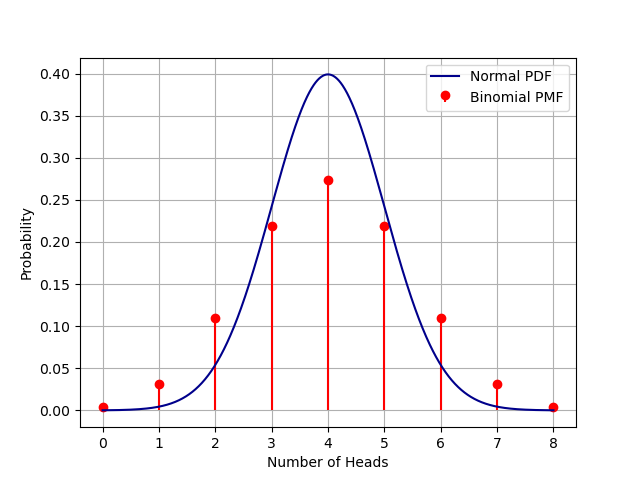
\includegraphics[width=\columnwidth]{./figs/fig.png}
\caption{Binomial distribution vs Gaussian distribution}
	\label{fig58:_9_3_31}
\end{figure}
\item \textbf{Using Q function:}
\begin{align}
	Y \sim \gauss{\mu}{\sigma^2}
\end{align}
CDF of Y is given by
\begin{align}
	F_Y(y) &= 1 - \Pr(Y>y)\\
	&= 1 - \Pr\biggl(\frac{Y-\mu}{\sigma}>\frac{y-\mu}{\sigma}\biggr)
\end{align}
As
\begin{align}
	\frac{Y-\mu}{\sigma} \sim \gauss{0}{1}\\
	\implies F_Y(y) = 1 - Q\biggl(\frac{y-\mu}{\sigma}\biggr)
\end{align}
including a correction upto 0.5,
\begin{align}
	p_Y(2.5<Y<3.5) & = F_Y(3.5) - F_Y(2.5)\\
	&= Q\biggl( \frac{2.5-\mu}{\sigma} \biggr) - Q\biggl( \frac{3.5-\mu}{\sigma} \biggr)\\
	&= Q(-1.0608) - Q(-0.3536)\\
	&= 0.855610 - 0.638181\\
	&= 0.1974
\end{align}

\item \textbf{Comparing all three techniques:}\\
\begin{table}[H]
\def\arraystretch{1.2}
\begin{tabular}{|c|c|c|c|}
	\hline
	\textbf{Event} &\textbf{Binomial} &\textbf{Gaussian} &\textbf{Q function}\\ 
	\hline
	Getting exactly 3 heads &0.21875 &0.35206 &0.1974\\ 
	\hline
\end{tabular}
\end{table}
\end{enumerate}
\end{document}
